\documentclass{standalone}
\usepackage{tikz,pgfplots}
\pgfplotsset{compat=1.18}
\begin{document}
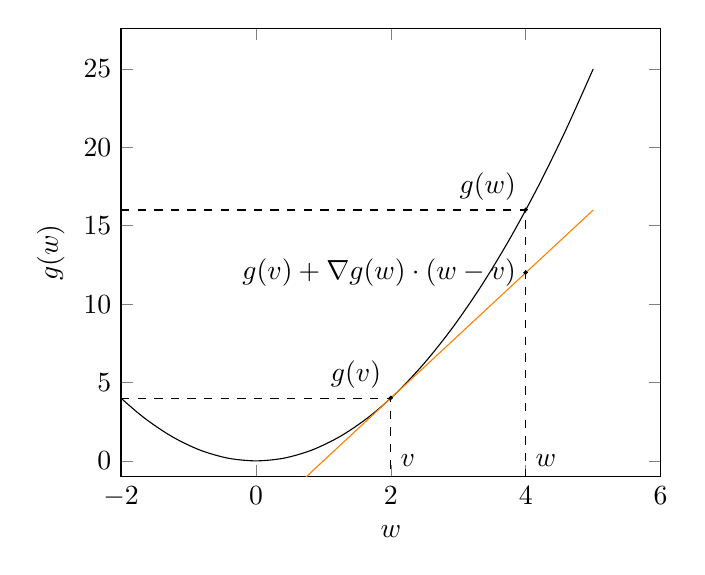
\begin{tikzpicture}
\begin{axis}[
        xlabel=$w$,
        ylabel=$g(w)$,
        xmin=-2,xmax=6,
        ymin=-1
        ]
    \addplot[smooth]{x^2};
    \addplot[smooth,orange]{4*x-4};
    \draw[dashed](-2,4)--(2,4)node[draw,circle,fill=black, inner sep=0.5pt]{}node[above left]{$g(v)$}--(2,-1)node[above right]{$v$};
    \draw[dashed](-2,16)--(4,16)node[draw,circle,fill=black, inner sep=0.5pt]{}node[above left]{$g(w)$}--(4,12)node[draw,circle,fill=black,inner sep=0.5pt]{}node[left]{$g(v)+\nabla g(w)\cdot(w-v)$}--(4,-1)node[above right]{$w$};
\end{axis}    
\end{tikzpicture}
\end{document}